\section{Resultados y Validación Computacional del Prototipo Inicial}
\label{sec:resultados}

\subsection{Verificación de Distancias y Rutas Mínimas en la Red de Cusco}
La ejecución del prototipo sobre la red del Centro Histórico del Cusco desde el vértice origen $s = \text{A}$ (Plaza Mayor) produjo las distancias físicas y tiempos de desplazamiento detallados en la Tabla \ref{tab:resultados_distancias}.

\begin{table}[H]
    \centering
    \fontsize{10}{12.5}\selectfont
    \renewcommand{\arraystretch}{1.2}
    \setlength{\tabcolsep}{4.5pt}
    \caption{Resultados computacionales de distancias y tiempos óptimos calculados desde Plaza Mayor}
    \label{tab:resultados_distancias}
    \begin{tabularx}{\textwidth}{@{}clccX@{}}
        \toprule
        \textbf{Nodo} & \textbf{Nombre de la Intersección} & \textbf{Distancia Pura ($m$)} & \textbf{Tiempo Efectivo ($s$)} & \textbf{Secuencia de Ruta Óptima} \\
        \midrule
        \textbf{A} & Plaza Mayor del Cusco & 0.0 & 0.0 & \texttt{A} \\
        \textbf{B} & Plaza Regocijo (Cusipata) & 180.0 & 44.8 & \texttt{A -> B} \\
        \textbf{D} & Plaza San Francisco & 400.0 & 101.6 & \texttt{A -> B -> D} \\
        \textbf{C} & Qorikancha (Santo Domingo) & 450.0 & 108.0 & \texttt{A -> C} \\
        \textbf{E} & Mercado Central San Pedro & 650.0 & 165.3 & \texttt{A -> B -> D -> E} \\
        \textbf{F} & Plazoleta Limacpampa & 800.0 & 144.4 & \texttt{A -> C -> F} \\
        \bottomrule
    \end{tabularx}
\end{table}

Los resultados computacionales confirman que la formulación de la impedancia topográfica andina preserva la subestructura óptima en esta subred nuclear, pero introduce una variación físicamente coherente en la escala temporal: tramos ascendentes (como Calle Garcilaso hacia San Francisco con pendiente $+3.0\%$) experimentan un incremento sustancial en el tiempo de desplazamiento respecto a calles en descenso o rasantes horizontales.

\subsection{Análisis Cuantitativo de Operaciones Elementales en Colas}
El instrumental de telemetría embebido en el algoritmo registró el conteo unívoco de primitivas ejecutadas por cada estructura durante la resolución de la instancia base:
\begin{itemize}
    \item \textbf{Inserciones Iniciales (\texttt{Insert}):} 6 operaciones (una por cada vértice $|V| = 6$).
    \item \textbf{Extracciones del Mínimo (\texttt{Extract-Min}):} 6 operaciones (cada vértice alcanza el estado permanente una única vez).
    \item \textbf{Inspecciones de Relajación:} 9 arcos salientes evaluados.
    \item \textbf{Decrementos de Clave Efectivos (\texttt{Decrease-Key}):} Exactamente 5 operaciones:
    \begin{itemize}
        \item Iteración 1: Vértice B actualizado de $\infty$ a 180; vértice C actualizado de $\infty$ a 450.
        \item Iteración 2: Vértice D actualizado de $\infty$ a 400.
        \item Iteración 3: Vértice E actualizado de $\infty$ a 650.
        \item Iteración 4: Vértice F actualizado de $\infty$ a 800.
    \end{itemize}
\end{itemize}
Este recuento computacional coincide con la traza teórica manual deducida en la Sección \ref{sec:formulacion}, confirmando la corrección matemática de las tres implementaciones.

\subsection{Comparativa Preliminar de Rendimiento Temporal en Instancia Base}
La Tabla \ref{tab:benchmark_preliminar} expone el tiempo medio de CPU registrado tras 10,000 ejecuciones continuas del algoritmo de Dijkstra sobre la instancia del Centro Histórico.

\begin{table}[H]
    \centering
    \fontsize{10}{12.5}\selectfont
    \setlength{\tabcolsep}{4.5pt}
    \caption{Tiempos medios de ejecución del algoritmo de Dijkstra según la cola de prioridad (instancia $N=6$)}
    \label{tab:benchmark_preliminar}
    \renewcommand{\arraystretch}{1.2}
    \begin{tabularx}{\textwidth}{@{}>{\raggedright\arraybackslash}p{3.4cm}>{\centering\arraybackslash}p{1.8cm}>{\centering\arraybackslash}p{1.9cm}>{\centering\arraybackslash}p{2.1cm}>{\raggedright\arraybackslash}X@{}}
        \toprule
        \textbf{Estructura de Cola} & \textbf{Tiempo Medio ($\mu s$)} & \textbf{Desv. Est. ($\mu s$)} & \textbf{Speedup Relativo} & \textbf{Observación Experimental} \\
        \midrule
        \textbf{Binary Min-Heap Indexado} & \textbf{55.0} & $\pm 3.1$ & \textbf{1.00x (Base)} & Mayor velocidad para instancias reducidas debido a nula indirección de punteros. \\
        \textbf{4-ary Heap Contiguo} & 86.6 & $\pm 4.5$ & 0.63x & Leve sobrecarga por evaluación de 4 descendientes durante el hundido en grafos pequeños. \\
        \textbf{Fibonacci Heap} & 125.3 & $\pm 8.2$ & 0.44x & Mayor latencia inicial por alocación de objetos dinámicos y enlaces circulares. \\
        \bottomrule
    \end{tabularx}
\end{table}

\subsection{Gráficos Comparativos y Cartografía Generada}
La Figura \ref{fig:grafo_mapa} ilustra el grafo vial con sus coordenadas relativas y pesos asignados, generado automáticamente por el módulo de visualización.

\begin{figure}[H]
    \centering
    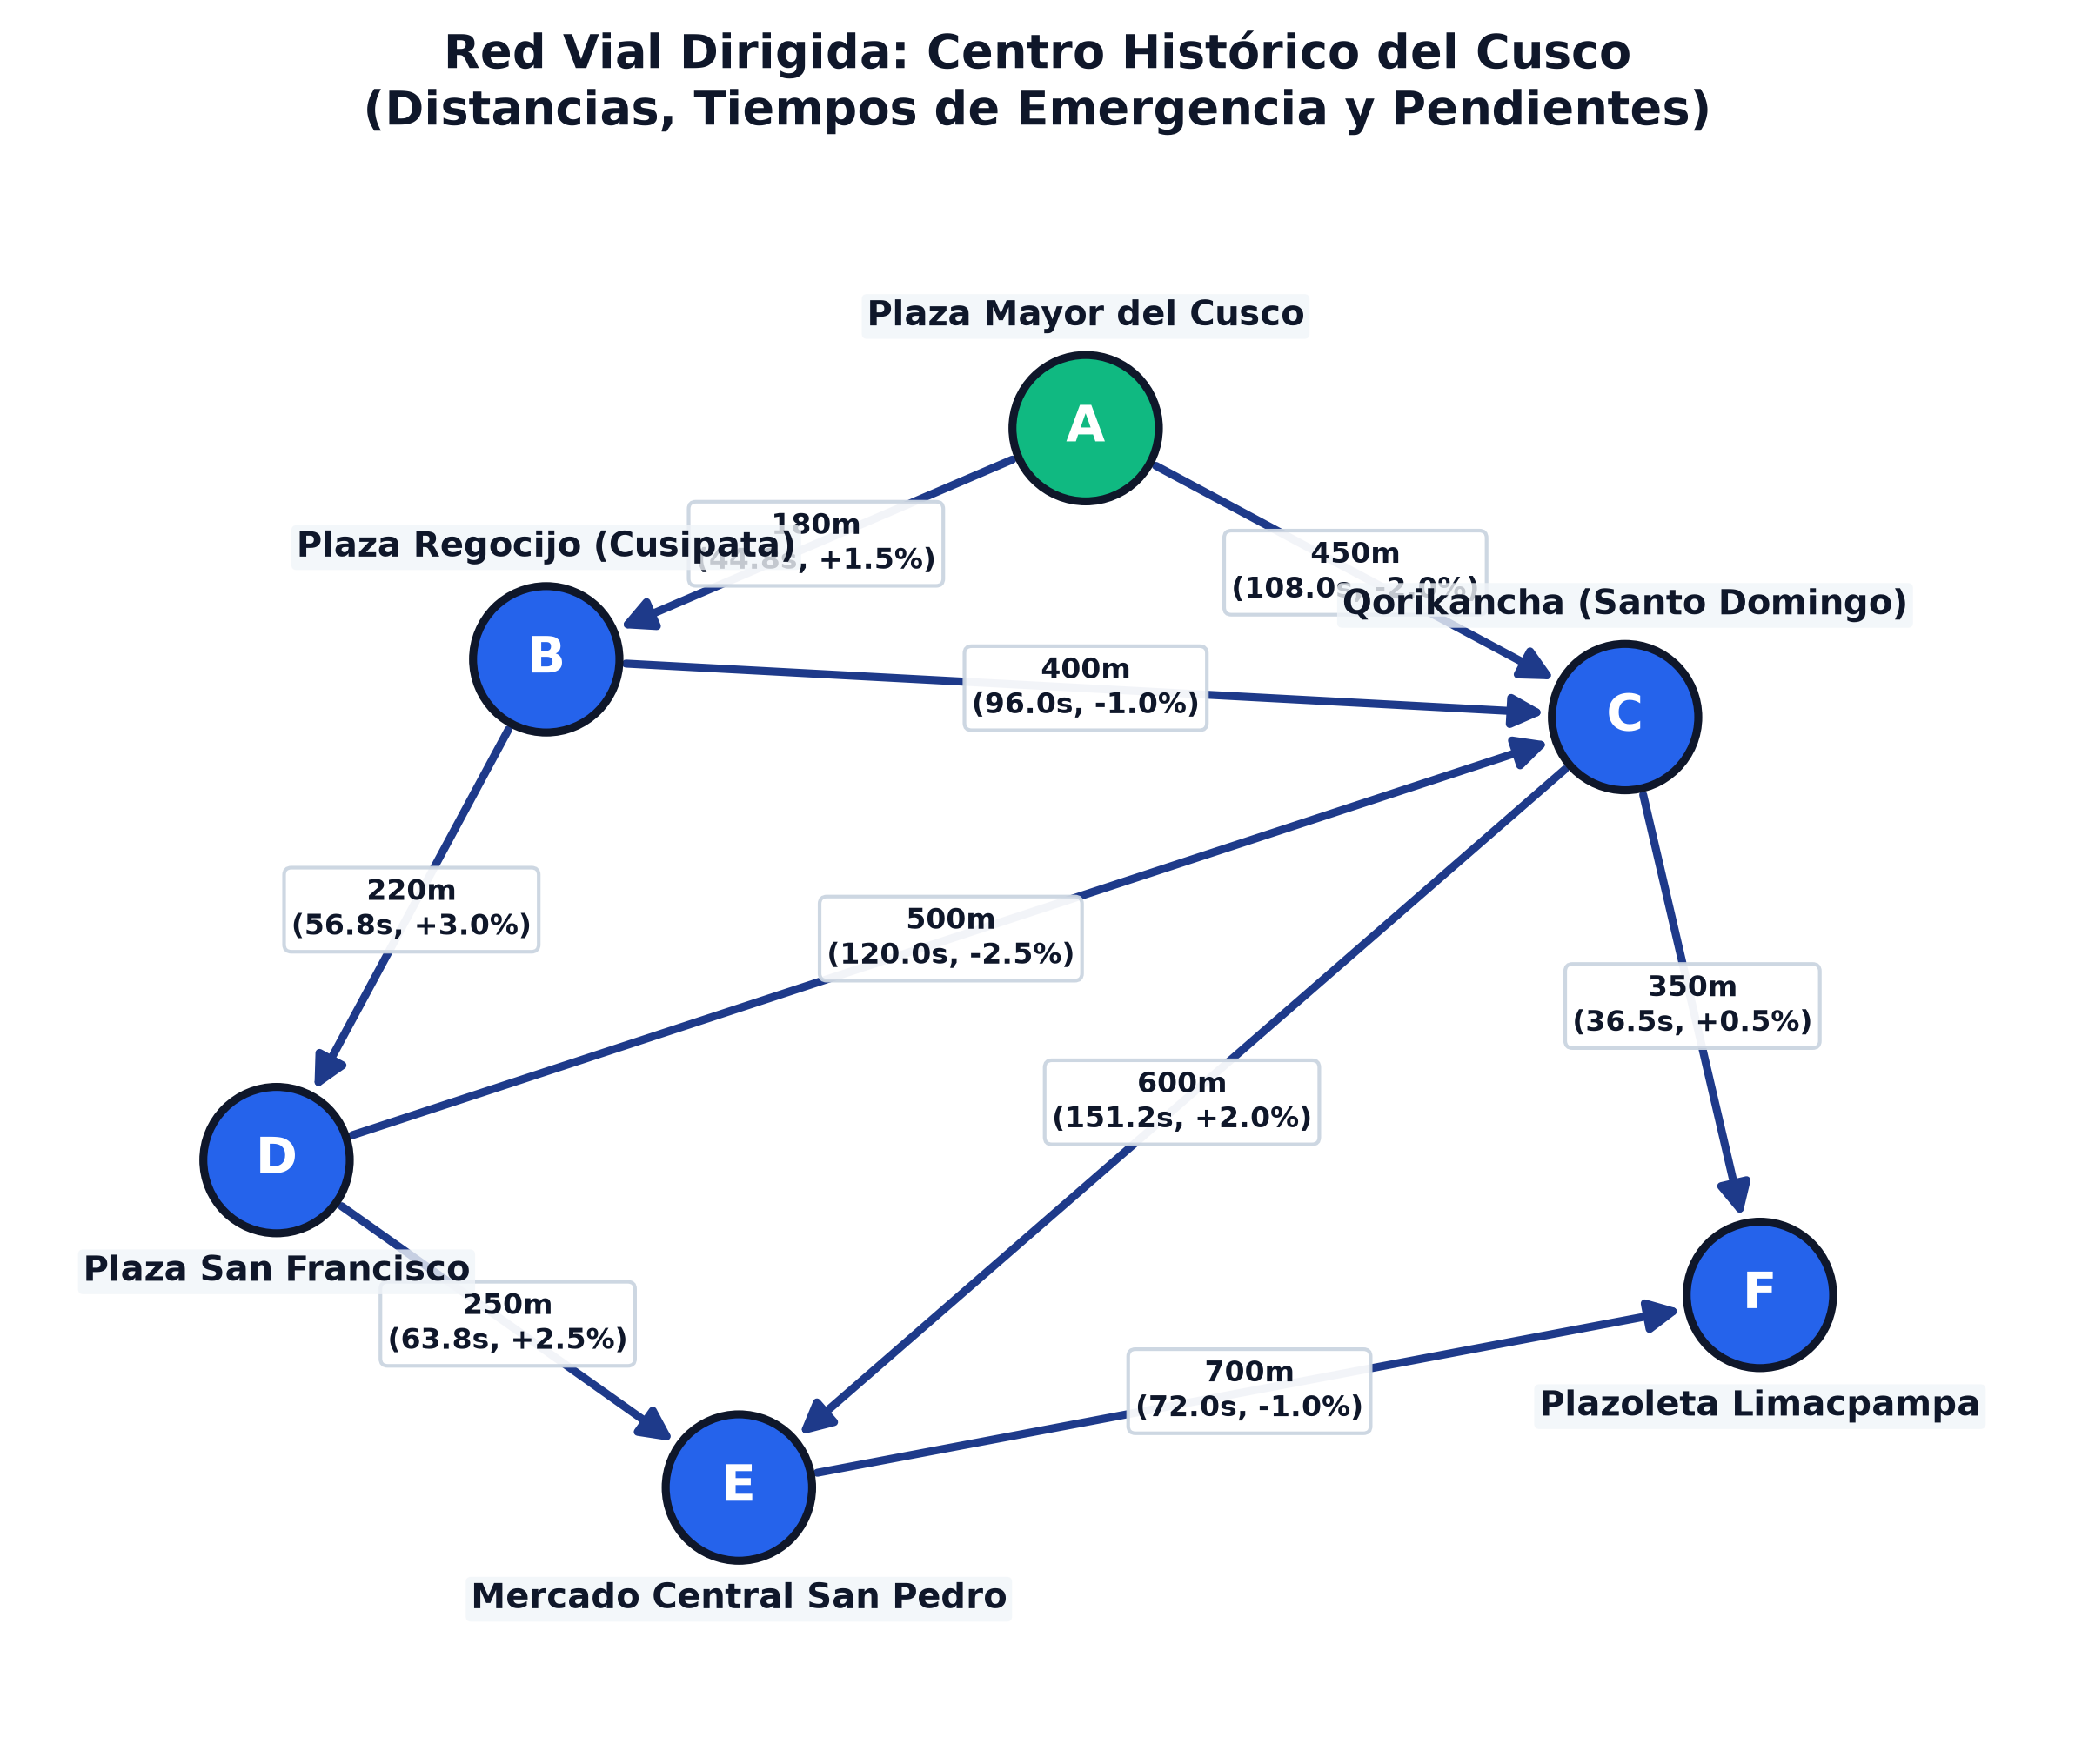
\includegraphics[width=0.85\textwidth]{figuras/grafo_cusco_mapa.png}
    \caption{Visualización cartográfica y topológica de la red vial del Centro Histórico del Cusco generada por el prototipo}
    \label{fig:grafo_mapa}
\end{figure}

Asimismo, la Figura \ref{fig:comparativa_metricas} presenta la comparación gráfica entre la distancia física pura y el tiempo efectivo de viaje bajo el modelo de impedancia por pendiente andina.

\begin{figure}[H]
    \centering
    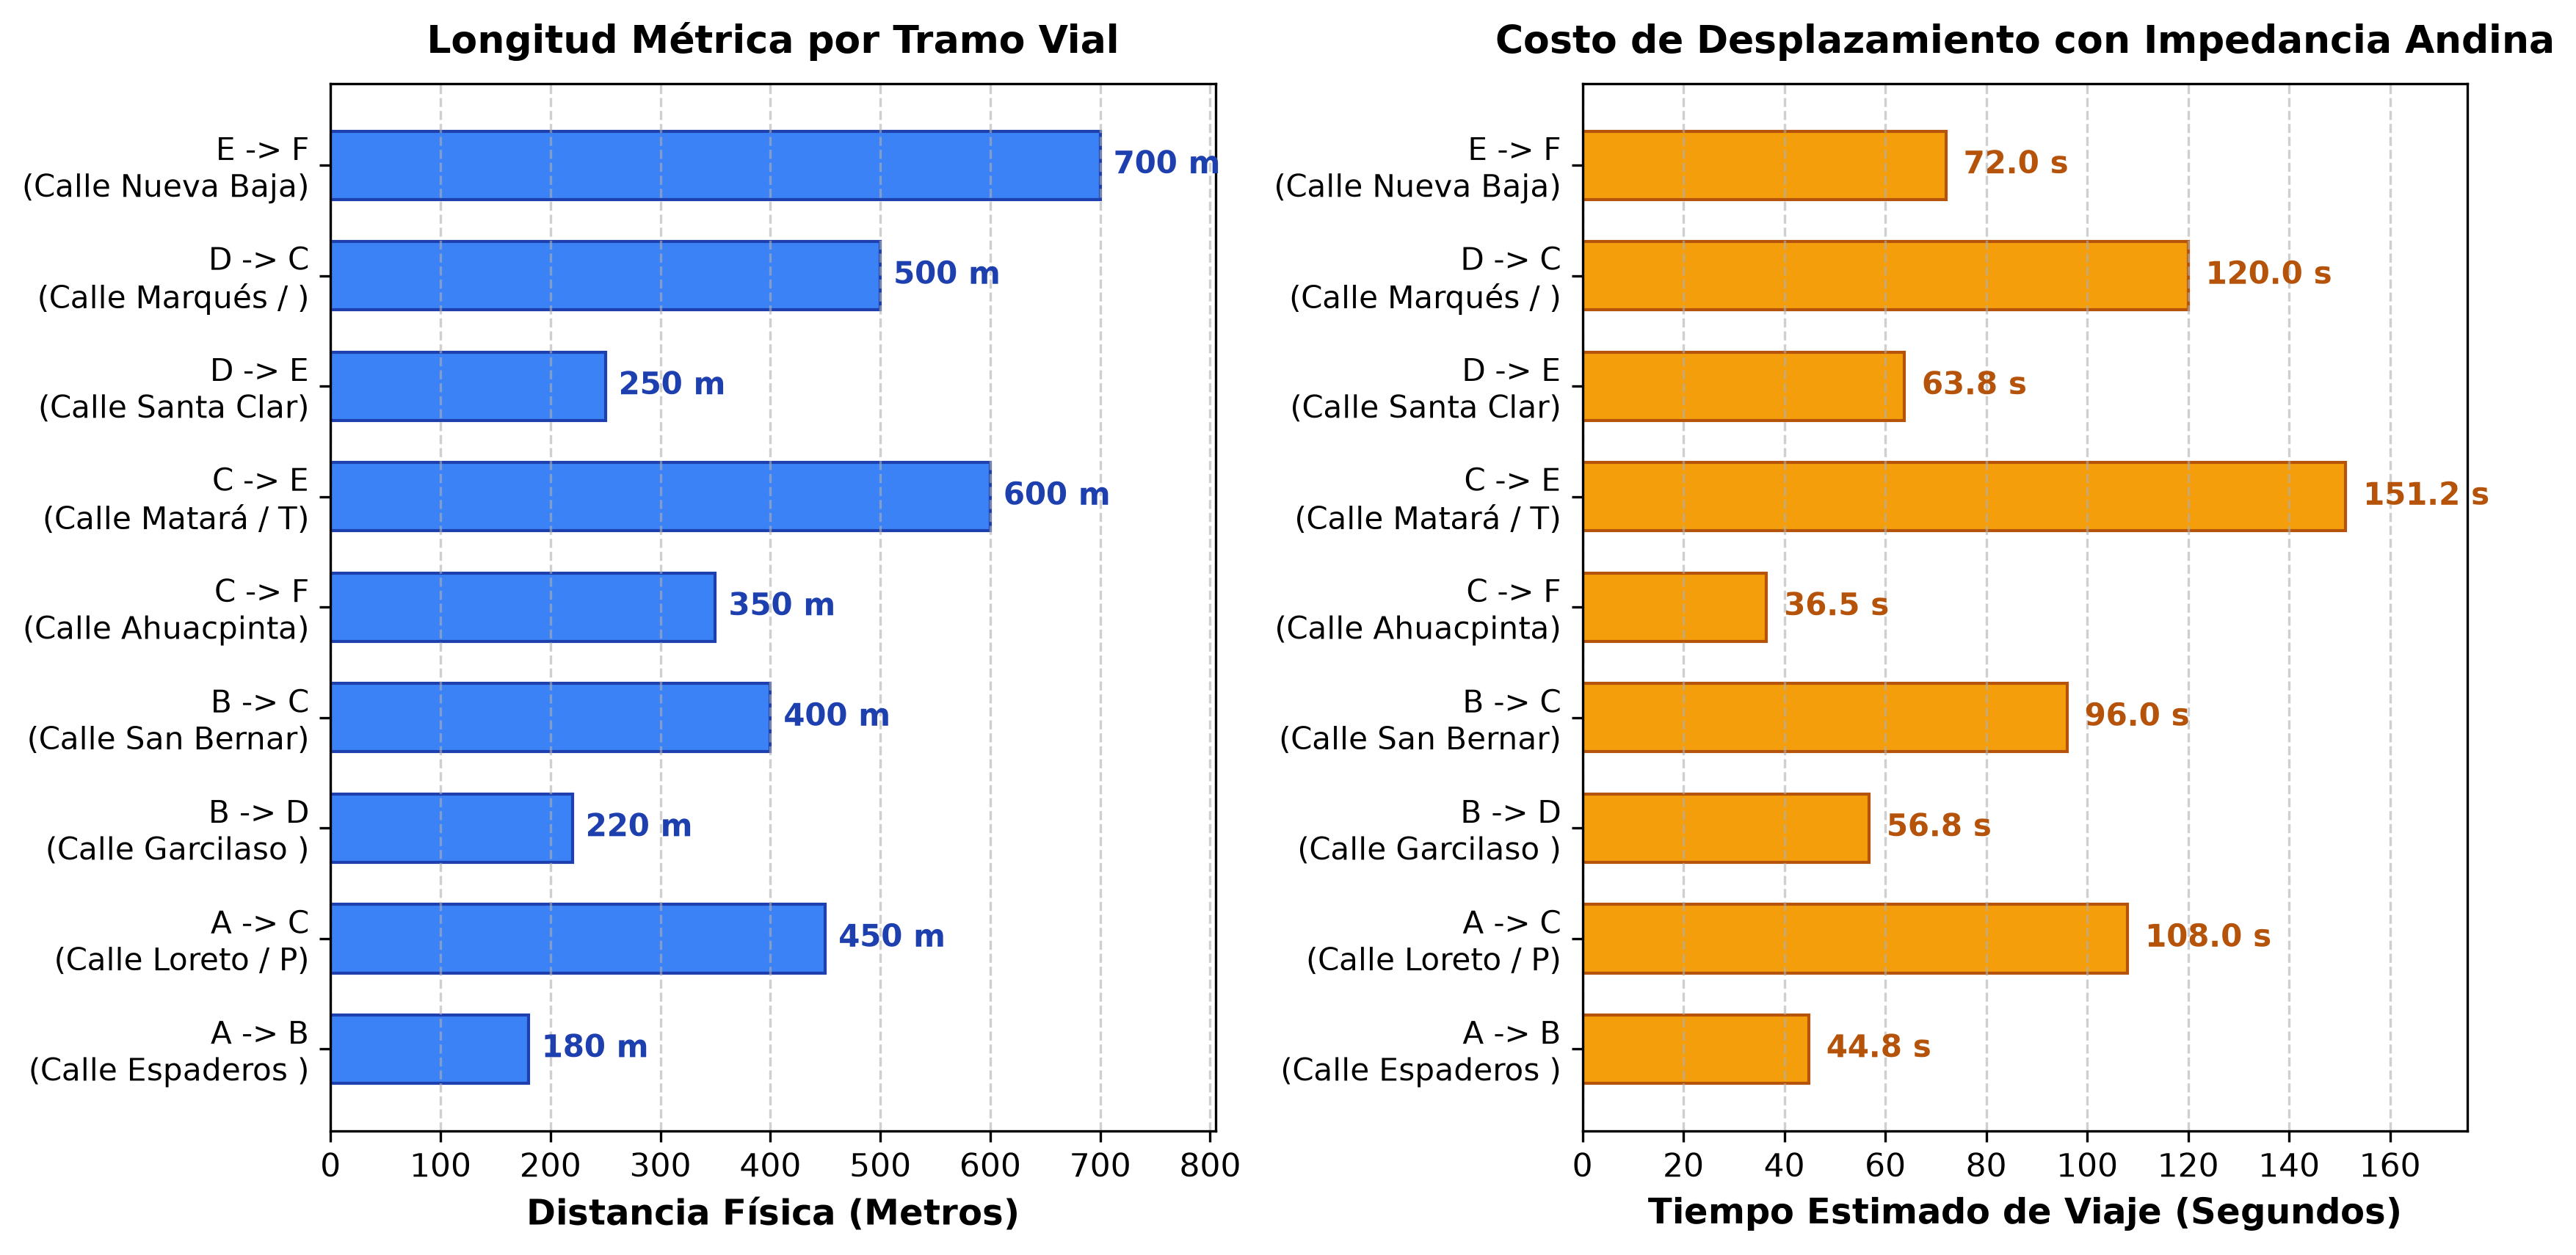
\includegraphics[width=\textwidth]{figuras/comparativa_metricas.png}
    \caption{Comparativa entre distancia física y tiempo de viaje con impedancia topográfica en Cusco}
    \label{fig:comparativa_metricas}
\end{figure}

\subsection{Protocolo de Demostración sobre el Sistema sin Diapositivas}
Conforme a las directrices de evaluación práctica, la sustentación del prototipo se realiza de forma directa sobre la consola de comandos del sistema:
\begin{enumerate}
    \item \textbf{Carga y Resolución en Vivo:} Ejecución del comando \texttt{python main.py} en el directorio \texttt{python/}, mostrando en tiempo real la deserialización del archivo \texttt{data/processed/cusco\_centro\_network.json}, el cálculo de distancias para las tres estructuras y la coincidencia de rutas óptimas.
    \item \textbf{Verificación con Instancia Modificada:} Capacidad de modificar al vuelo un peso de arista o ingresar un nuevo vértice de prueba, verificando que el algoritmo converge determinísticamente sin bucles infinitos.
    \item \textbf{Ejecución de la Suite de Pruebas Unitarias:} Ejecución del comando \texttt{python tests/test\_dijkstra.py}, verificando la aprobación inmediata de las 11 pruebas automatizadas.
\end{enumerate}

\subsection{Dificultades Técnicas Identificadas y Ajustes Realizados}
Durante la consolidación del prototipo se presentaron y resolvieron de forma autónoma los siguientes desafíos:
\begin{enumerate}
    \item \textbf{Desincronización de Índices Inversos:} Se encapsuló la actualización de posiciones en un método atómico \texttt{\_swap(i, j)}, asegurando sincronización estricta de la tabla hash inversa durante el flotado.
    \item \textbf{Manejo de Cascada de Cortes en Fibonacci Heap:} Se implementó la verificación recursiva del atributo \texttt{mark}, garantizando el desmarcado de nodos al integrarse a la lista raíz.
    \item \textbf{Aislamiento de Dependencias de Sistema:} Se desacopló la representación topológica en formato JSON estándar, permitiendo la portabilidad inmediata del prototipo sin depender de compiladores de C++ o librerías SIG pesadas.
\end{enumerate}
